\section{The Probabilistic Approach}


\subsection{Probabilistic Knowing How with Linear Plans}
Naturally, our first approach will be extending $\Khlogic$ with some form of probabilistic behaviour. 

% We will start by introducing PLTS, an extension of LTS with probabilities.

% \begin{definition}\label{def:plts}
%     Let $\PROP$ be a countable set of propositional symbols. 
%     A \emph{Probabilistic Labeled Transition System (PLTS)}  is a tuple
%     $\model=\tup{\S,\ACT,\ra,\V}$, defined exactly as an LTS except that ${\ra}\subseteq \S \times \ACT \times \dist(\S)$, where  $\dist(\S)$ is the set of probability distributions over $\S$.
% \end{definition}

% We will start by introducing PLTS, an extension of LTS with probabilities.

% \begin{definition}\label{def:plts}
%     Let $\PROP$ be a countable set of propositional symbols. 
%     A \emph{Probabilistic Labeled Transition System (PLTS)}  is a tuple
%     $\model=\tup{\S,\ACT,\ra,\V}$, defined exactly as an LTS except that ${\ra}\subseteq \S \times \ACT \times \dist(\S)$, where  $\dist(\S)$ is the set of probability distributions over $\S$.
% \end{definition}

\begin{figure}[t]
    \begin{center}
        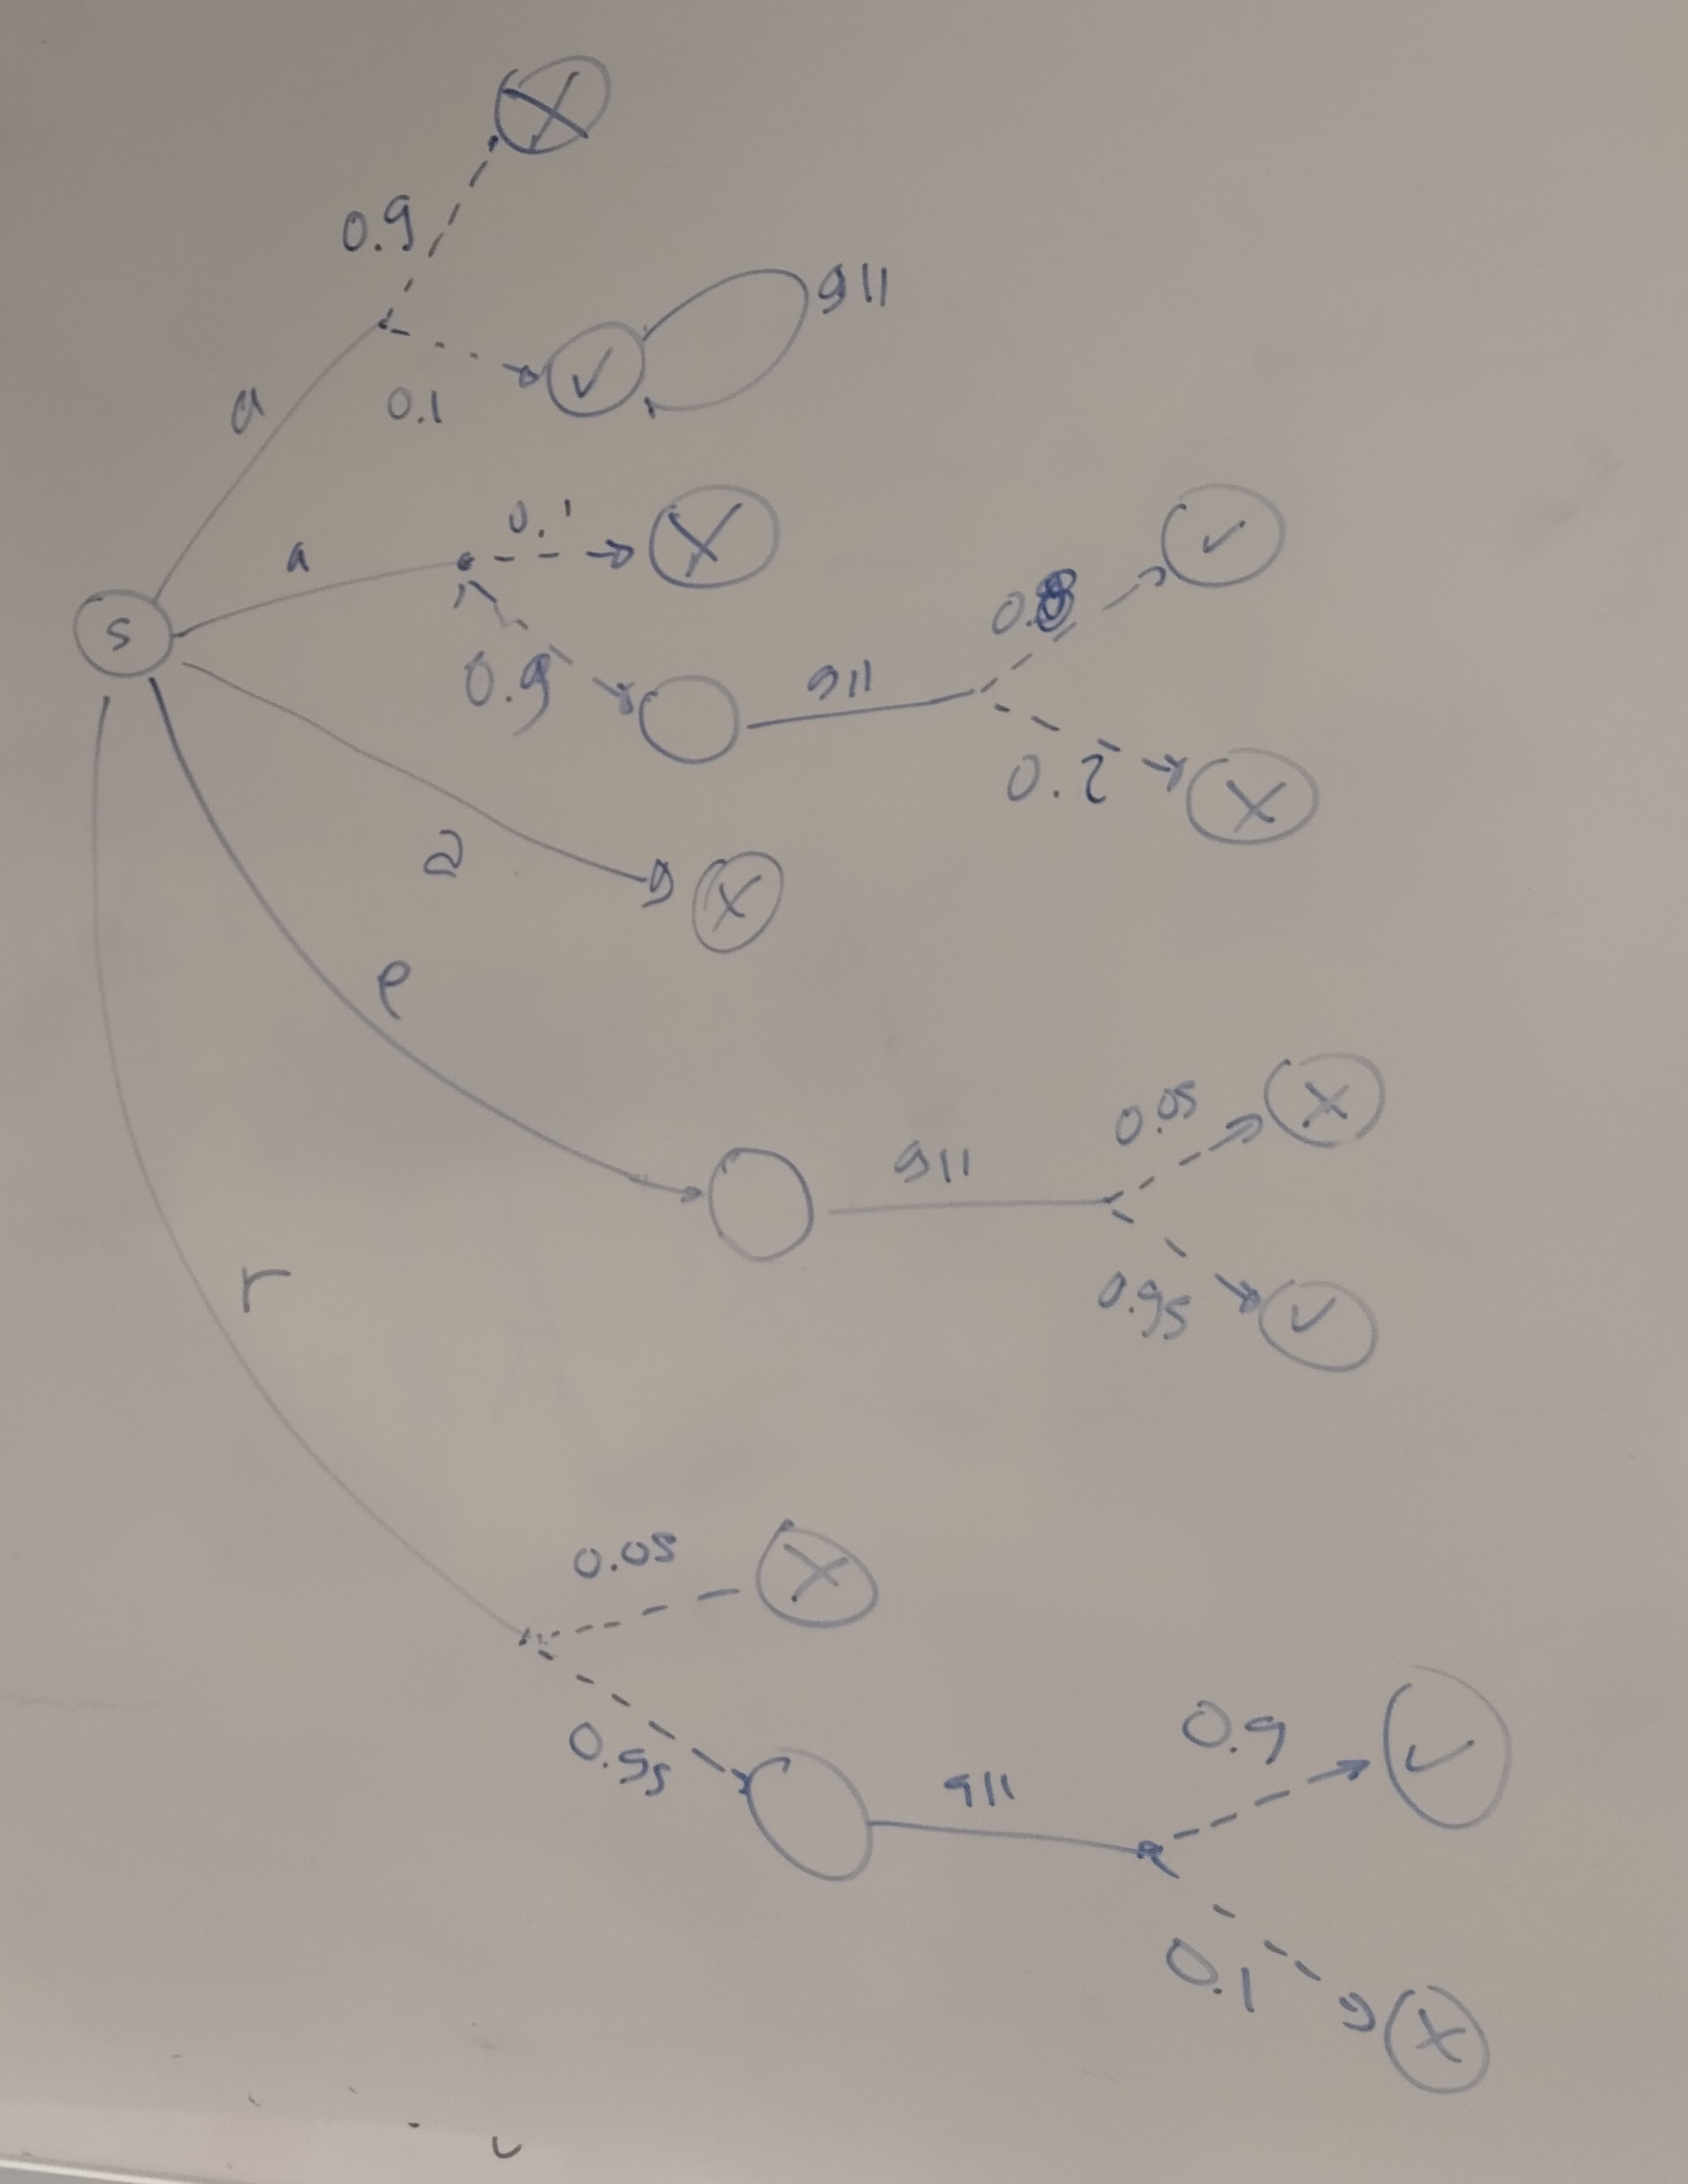
\includegraphics[scale=0.1]{PLTS.jpg}
    \end{center}
\end{figure}

% We need to capture the notion of executability with probability at least $q$, for some $q\in[0,1]$. 

% \begin{definition}\label{def:strategy-comp-exec}
%     Let $\model=\tup{\S,\ACT,\ra,\V}$ be a PLTS, a \emph{strategy} is a function $\strat: \S\times(\ACT\times\S)^* \ra \dist(\S\times\ACT\times\dist(\S))$. Let $\plan\in\ACT^*$, we say that $\strat$ is \emph{$\plans$-compatible} if and only if, for all $\rho\in \S\times(\ACT\times\S)^*$, the following conditions hold:
%     \begin{enumerate}
%         \item $\strat(\rho)(s,a,\mu)>0$ implies $\last(\rho)=s$ and $s\reach{a}\mu$ in $\model$, and 
%         \item $\bar{\rho}\in\pref(\plans)$ implies $\bar{\rho}a\in\pref(\plans)$.
%     \end{enumerate}
%     For $\plan\in\ACT^*$, we say that $\sigma$ is \emph{$\plan$-compatible} if it is $\{\plan\}$-compatible. 

%     Let $q\in[0,1]$, we say that $\plans$ is \emph{$q$-executable} at $s\in\S$, if and only if, 
%     \[
%         \infim_{\{\strat \mid \strat \text{ is } \plans\text{-comp.}\}} \Prob^\strat_{s}(\plans)\geq q.
%     \]
%     Finally, $\plans$ is \emph{$q$-executable} at $B\subseteq\S$, if and only if, it is $q$-executable at every $s\in B$. 
%     A plan $\plan$ is \emph{$q$-executable} at $s$ (respectively, at $B$) if $\{\plan\}$ is $q$-executable at $s$ (respectively, at $B$). 
% \end{definition}

% \bigpedro{todo lo de arriba en esta subsecci\'on deber\'ia irse, la mayor\'ia de las cosas est\'an definidas en los preliminaries, queda la idea de $\plans$-compatible que viene debajo}



Given a set of plans $\plans\subseteq\ACT^*$, we want to consider
strategies that follow as faithfully as possible the plans of
$\plans$.  Therefore, we say that a strategy $\sigma$ is
\emph{$\plans$-compatible} if for all $\rho\in\execf$ such that
$\bar{\rho}\in\pref(\plans)$,
%
\begin{enumerate}
\item%
  $\strat(\rho)(a,\mu)>0$ implies $\bar{\rho}a\in\pref(\plans)$, and
\item%
  $\strat(\rho)(\complete)>0$ implies that either
  $\bar{\rho}\in\plans$ or
  $\bar{\rho}\{a\mid{\last(\rho)\reach{a}\mu}\}\cap\pref(\plans) = \emptyset$. 
\end{enumerate}
%
The first item states that $\strat$ can chose an $a$-labelled
transition after the partial plan $\bar{\rho}$ if the continuation of
$\bar{\rho}a$ is also a partial plan.
%
The second item states that $\strat$ is allowed to terminate after the
partial plan $\bar{\rho}$ if either $\bar{\rho}$ is itself a valid
plan, or $\bar{\rho}$ cannot be continued by the PLTS within some
valid plan.
%
Let $\Comp(\plans)$ denote the set of all $\plans$-compatible
strategies.
%
%% Given a plan $\plan\in\ACT^*$, we say that a strategy $\strat$ is
%% $\plan$-compatible iff it is $\{\plan\}$-compatible.
\pedro{poner ejemplos de $\plans$-compatible respecto de alg\'un running
  example}


Let $\plans$ be a set of plans that are believed to perform
equivalently in order to reach some goal state in $G\subseteq\S$.  We
define the set of \emph{successful complete (finite) execution} that
reach $G$ following some plan in $\plans$ by
$\Succ(\plans,G)=\{{\rho\complete\in\cexecf}\mid{\bar{\rho}\in\plans
  \text{ and } \last(\rho)\in G}\}$.
%
We are interested in that any $\plans$-compatible strategy $\sigma$
starting from a given state $s\in\S$ reaches a state in $G$ with a
minimum desired probability, say $q$.  That is, we would like that
%
\begin{equation}\label{eq:plans:goal:q}
  \inf_{\sigma \in\Comp(\plans)}\Prob^\strat_s(\Succ(\plans,G)) \geq q.
\end{equation}
%
More generally, we would like that this holds from any particularly
assumed state in a set $A\subseteq\S$ (say, a precondition).  So, we
write $A \reach{\plans}_q G$ if and only if for all state $s\in A$,
the condition in \cref{eq:plans:goal:q} holds.
%
Thus $A \reach{\plans}_q G$ means that any state in $A$ can reach the
goal $G$ with at least probability $q$ following some plan in $\plans$
\textcolor{red}{in an adaptively manner}.
\pedro{ejemplo de esto tambi\'en}


\bigpedro{creo que es importante pensar ahora la estructura del paper}




\bigpedro{desde el cartel hasta aqu\'i es nuevo}



Notice that, whenever $q=1$, we are in the case of SE from~\Cref{def:plans}. \raul{Chequear esto} The extended language with probabilities is given below.


\begin{definition}
    \label{def:syntax-extended}
    The set of formulas (a.k.a. the language) of $\Khlogic$ is defined by the following BNF:
    \[
        \varphi, \psi ::= p \mid \neg \varphi \mid \varphi \vee \psi \mid \kh^q(\psi,\varphi),
    \]
    where $p\in\PROP$ and $q\in[0,1]$. Other Boolean operators are defined as usual. Formulas of the form $\kh(\psi,\varphi)$ are read as \emph{``the agent knows how to achieve $\varphi$ given $\psi$ with probability at least $q$''}.
\end{definition}




Now we proceed by introducing the semantics of the new modality.

\begin{definition}
    Let $\model = \tup{\S,\ACT,\ra,\V}$ be a PLTS and let $s\in\S$, the satisfiability relation $\models$ for $\PKh$ is inductively defined as:
    \[
        \begin{array}{l@{\ \ \ }c@{\ \ \  }l}
        % \model, s \models p & \iffdef & p \in \V(s) \\
        % \model, s\models \neg\varphi & \iffdef & \model, s \not\models \varphi \\
        % \model, s \models \psi\vee\varphi & \iffdef & \model, s \models \psi \mbox{ or }\model, w \models \varphi \\
        \model, s \models \kh^q(\psi,\varphi) & \iffdef & \text{there is } \plan \in \ACT^* \;\text{such that:} \\
        & & \ \ \text{\rm (1)} \ \plan \text{ is $q$-executable at }  \truthset{\model}{\psi}\; \text{and} \\
        & & \ \ \text{\em (2)} \ \truthset{\model}{\psi} \reach{\plan}_q \truthset{\model}{\varphi}, 
        \end{array}
        \] \raul{1 and 2 will be merged into one condition.}
        where: $\truthset{\model}{\chi} := \csetsc{s\in\S}{\model,w\models\chi}$. Define: $\model\models\varphi$ iff  $\truthset{\model}{\varphi}=\S$, and $\models\varphi$ iff $\model\models\varphi$, for all PLTS $\model$.
\end{definition}

\begin{theorem}\label{th:mc-khp-undecidable}
The model-checking problem for $\PKh$ is undecidable.
\end{theorem}

\begin{proof}
    Suppose we want to check whether $\model,s\models\kh^q(\psi,\varphi)$.  W.l.o.g., consider $\model$ is complete and deterministic. 
    From the semantics, we need to check if there is $\plan\in\ACT^*$ satisfying conditions (1) and (2). Consider condition (1), i.e., we need to check whether $\plan$ is $q$-executable at all $s\in\truthset{\model}{\psi}$. Fix such an $s$. Since $\model$ is deterministic and complete, it all boils down to check whether there is $\plan\in\ACT^*$ such that $\Prob^\strat_s(\plan)\geq q$ (notice that $\strat$ is unique by determinism of $\model$). 
    The latter solves the problem of checking whether the language recognized by a probabilistic (deterministic) automata is empty, which is undecidable~\cite{MadaniHC99}. 
\end{proof}


\subsection{A First Approach: Non-Adaptable Plans}

The results in the above show a huge jump in the computational behaviour of knowing-how: while model-checking in the standard case is \PSPACE-complete, considering probabilities leads to undecidability of the same problem. Here, we will deal with the version of knowing-how, in which an agent only considers plans that belong to its uncertainty/awareness class. We will introduce two logics considering probabilities, one generalizing the logic from~\cite{AFSVQ21,AFSVQ23} (each plan in a class must be an appropriate plan) and another one in which it will suffice to have certain appropriate plans in a class. For the former, the model-checking problem again becomes undecidable (contrary to the \PTIME problem of the logic without probabilities, see e.g.~\cite{AFSVQ21,AFSVQ23,DF23}), while for the second, the problem is decidable. In what follows, apart from the technical results, we will motivate the use of the decidable logic in some examples.

Here we introduce some definitions, extending those in e.g.~\cite{AFSVQ21,AFSVQ23}.


\begin{definition}\label{def:plts}
    Let $\PROP$ be a countable set of propositional symbols and let $\AGT$ be a finite set of agents.  
    A \emph{Probabilistic Labeled Transition System with uncertainty (PLTSU)}  is a tuple
    $\model=\tup{\S,\ACT,\ra,\sim,\V}$ s.t. $\tup{\S,\ACT,\ra,\V}$ is a PLTS, and 
    \begin{itemize}
        % \item $\S$ is a countably non-empty set of states,
        % \item $\ACT$ is a countable set of action symbols,
        % \item $\dist(\S)$ is the set of probability distributions over $\S$,
        % \item ${\ra} \subseteq \S \times \ACT \times \dist(\S)$ is a transition relation,
        \item ${\sim}\subseteq \DS{}\times \DS{}$ (where $\DS{}\subseteq\ACT^*$) is an equivalence relation over $\DS{}$. 
        % \item $\V: \S \ra 2^\PROP$ is a valuation function.
    \end{itemize}
    %Elements of $\ACT^*$ are called \emph{plans}, and 
    Each $\sim$ is called the indistinguishability relation between plan. 
    % We write $\plan\sim_i\plan'$ whenever $(\plan,i,\plan')\in{\sim}$, and we define $\DS{i}:=\set{\plan \mid \text{ there is } \plan' \text{ s.t. } \plan\sim_i\plan'}$. 
    By $[\plan]_{\sim}:=\set{\plan' \in \DS{} \mid \plan \sim_i \plan'}$ we denote $\plan$'s equivalence relation with respect to $\DS{}$, then we define the \emph{indistinguishability set of $\model$} as $\Unc := \set{[\plan]_{\sim} \mid \plan\in\DS{}}$. 
    %The set $\Unc:=\set{\Unc(i) \mid i\in\AGT}$ is called the \emph{uncertainty set} of $\model$. 
    For simplicity sake, we sometimes denote $\model=\tup{\S,\ACT,\ra,\Unc,\V}$ to refer to a PLTS, i.e., we will use its uncertainty set instead of the indistinguishability relation.
\end{definition}

Notice that, as it is defined in~\cite{AFSVQ21,AFSVQ23}, $\Unc$ represents the perception the agent has about the reality. In turn, the relation $\sim$ is not an equivalence relation over $\ACT^*$ but over $\DS{}$, as the latter contains only the plans she considers available or suitable for her purposes, while those in $\ACT^*\setminus\DS{}$ are not considered by the agent, even if they are suitable plans. 

% \begin{definition} \label{def:executability} \raul{TBC}
%     Let  $\model=\tup{\S,\ACT,\dist(\S),\ra,\Unc,\V}$ be a PLTSU, let $\plan\in\ACT^*$ be a plan, and let $q\in[0,1]$ a probability, we need to define two notions:
%     \begin{enumerate}
%         \item We say $\plan$ is \emph{$q$-executable} at $s\in\S$ iff ...  Extend it for set of plans and set of states.
%         \item For $s,t\in\S$, we write $s \reach{\plan}_q t$ iff ... Extend it for set of plans and set of states.
%     \end{enumerate}
% \end{definition}

In general, we will assume that PLTS are complete, as for those we can always complete the execution of a plan to a \emph{sink state}.

% \begin{definition}
%     \label{def:syntax}
%     The set of formulas (a.k.a. the language) of $\PKhunc$ is defined by the following BNF:
%     \[
%         \varphi, \psi ::= p \mid \neg \varphi \mid \varphi \vee \psi \mid \kh_i^q(\psi,\varphi),
%     \]
%     where $p\in\PROP$, $i\in\AGT$ and $q\in[0,1]$. Other Boolean operators are defined as usual. Formulas of the form $\kh_i^q(\psi,\varphi)$ are read as \emph{``agent $i$ knows how to achieve $\varphi$ given $\psi$, with probability $q$''}
% \end{definition}

\begin{definition} \label{def:semantics-non-adap}
    Let $\model = \tup{\S,\ACT,\ra,\Unc,\V}$ be a PLTSU and let $s\in\S$, the satisfiability relation $\models$ for $\PKhunc$ is inductively defined as:
    \[
    \begin{array}{l@{\ \ \ }c@{\ \ \  }l}
    % \model, s \models p & \iffdef & p \in \V(s) \\
    % \model, s\models \neg\varphi & \iffdef & \model, s \not\models \varphi \\
    % \model, s \models \psi\vee\varphi & \iffdef & \model, s \models \psi \mbox{ or }\model, w \models \varphi \\
    \model, s \models \kh^q(\psi,\varphi) & \iffdef & \text{there is } \plans \in \Unc \;\text{such that for all } \plan\in\plans{:} \\
    & & \ \ \text{\rm (1)} \ \plan \text{ is $q$-executable at }  \truthset{\model}{\psi}\; \text{and} \\
    & & \ \ \text{\em (2)} \ \truthset{\model}{\psi} \reach{\plan}_q \truthset{\model}{\varphi}, 
    \end{array}
    \]     \raul{1 and 2 to be merge into one.}
    \noindent where: $\truthset{\model}{\chi} := \csetsc{s\in\S}{\model,w\models\chi}$. Define: $\model\models\varphi$ iff  $\truthset{\model}{\varphi}=\S$, and $\models\varphi$ iff $\model\models\varphi$, for all PLTS $\model$.
\end{definition}

This definition bears a resemblance to the one in Section~\ref{sec:khlinearplans}, except that we ask the conditions hold for \emph{every plan} belonging to a set of indistinguishable plans $\plans$. We call this version of the logic \emph{non-adaptable} for such a reason, as the agent cannot use the ``good plans'' whenever she considers them ``equally good'' as others.  We will discuss later an alternative to this notion.

For this logic, we obtain a result similar to the one in the previous section.

\begin{theorem}\label{th:mc-khp-nadapt-undecidable}
    The model-checking problem for $\PKhunc$ under the semantics from Definition~\ref{def:semantics-non-adap} is undecidable.
\end{theorem}


\subsection{A Second Approach: Adaptable Plans}

Now we introduce a version of the logic $\PKhunc$ in which suitable plans for achieving a goal are \emph{adaptable}, in the sense that the full set $\plans$ must be $q$-executable, and not each plan $\plan\in\plans$ separately. Thus, the agent can use those plans that are good for her purposes, even in presence of non-appropriate plans that she considers indistinguishable from the good ones. \raul{Esto hay que venderlo un poco mejor.}

\begin{definition} \label{def:semantics-adap}
    Let $\model = \tup{\S,\ACT,\ra,\Unc,\V}$ be a PLTSU and let $s\in\S$, the satisfiability relation $\models$ for $\PKhunc$ is inductively defined as:
    \[
    \begin{array}{l@{\ \ \ }c@{\ \ \  }l}
    % \model, s \models p & \iffdef & p \in \V(s) \\
    % \model, s\models \neg\varphi & \iffdef & \model, s \not\models \varphi \\
    % \model, s \models \psi\vee\varphi & \iffdef & \model, s \models \psi \mbox{ or }\model, w \models \varphi \\
    \model, s \models \kh^q(\psi,\varphi) & \iffdef & \text{there is } \plans \in \Unc \;\text{such that:} \\
    & & \ \ \text{\rm (1)} \ \plans \text{ is $q$-executable at }  \truthset{\model}{\psi}\; \text{and} \\
    & & \ \ \text{\em (2)} \ \truthset{\model}{\psi} \reach{\plans}_q \truthset{\model}{\varphi}, 
    \end{array}
    \]     \raul{1 and 2 to be merge into one.}
    \noindent where: $\truthset{\model}{\chi} := \csetsc{s\in\S}{\model,w\models\chi}$. Define: $\model\models\varphi$ iff  $\truthset{\model}{\varphi}=\S$, and $\models\varphi$ iff $\model\models\varphi$, for all PLTS $\model$.
\end{definition}

The general idea in condition 1 of the clause for $\kh$ establishes that all the plans in $\plans$ have a probablity of at least $q$ of succeeding. Since all plans in $\plans$ are indistinguishability, this needs to be guaranteed no matter which plan is chosen. However, there are at least two alternatives in this definition: one considering \emph{adaptability}, meaning that there is at least one possible execution of each plan in $\plans$ for which probability $q$ is guaranteed, and considering \emph{non-adaptability} whenever we need this guarantee on each possible execution of every plan in $\plans$. Condition 2 establishes that successfull states are reached with probability of at least $q$.

\begin{remark}
    Notice that an equivalence class $\plans$ can be defined in terms of a Deterministic Finite State Automata (DFA) $\mathcal{A}_{\plans}$. This way, the operation of checking $q$-executability can be perfomed over the product $\model\times\mathcal{A}_{\plans}$. In short, $\plans$ is $q$-executable at $s$ iff for each $\plan\in\plans$, there exists one MDP in  $\model\times\mathcal{A}_{\plans}$ in which the probability of executing $\plan$ is at least $q$. This will be used while designing a model-checking algorithm (connected with algorithms from~\cite{AFSVQ21,AFSVQ23,DF23}).
\end{remark}

\begin{theorem}\label{th:mc-khp-adapt-decidable}
    The model-checking problem for $\PKhunc$ under the semantics from Definition~\ref{def:semantics-adap} is decidable. Moreover, if each $\plans\in\Unc$ is given as input as a deterministic FSA, the problem is in $\PTIME$.
\end{theorem}